
\documentclass[review]{elsarticle}

\usepackage{lineno,hyperref}
\modulolinenumbers[5]

\journal{Nuclear Instruments and Methods B}

%%%%%%%%%%%%%%%%%%%%%%%
%% Elsevier bibliography styles
%%%%%%%%%%%%%%%%%%%%%%%
%% To change the style, put a % in front of the second line of the current style and
%% remove the % from the second line of the style you would like to use.
%%%%%%%%%%%%%%%%%%%%%%%

%% Numbered
%\bibliographystyle{model1-num-names}

%% Numbered without titles
%\bibliographystyle{model1a-num-names}

%% Harvard
%\bibliographystyle{model2-names.bst}\biboptions{authoryear}

%% Vancouver numbered
%\usepackage{numcompress}\bibliographystyle{model3-num-names}

%% Vancouver name/year
%\usepackage{numcompress}\bibliographystyle{model4-names}\biboptions{authoryear}

%% APA style
%\bibliographystyle{model5-names}\biboptions{authoryear}

%% AMA style
%\usepackage{numcompress}\bibliographystyle{model6-num-names}

%% `Elsevier LaTeX' style
\bibliographystyle{elsarticle-num}
%%%%%%%%%%%%%%%%%%%%%%%

\begin{document}

\begin{frontmatter}

\title{Liquid scintillator tiles for high radiation environments }


%% or include affiliations in footnotes:
\author[umd]{Alberto Belloni\corref{mycorrespondingauthor}}
\cortext[mycorrespondingauthor]{Corresponding author}
\ead{abelloni@umd.edu}
\author[umd]{Mahnegar Amouzegar}
\author[iowa]{Burak Bilki}
\author[umd]{Jeff Calderon}
\author[umd]{Sarah C. Eno}
\author[baylor]{Kenichi Hatakeyama}
\author[fnal]{James Hirschauer}
\author[umd]{Geng-Yuan Jeng}
\author[baylor]{Joseph Pastika}
\author[fnal]{Kevin Pedro}
\author[umd]{Joshua Samuel}
\author[elmer]{Elmer Sharp}
\author[umd]{Young Ho Shin}
\author[baylor]{Emrah Tiras}
\author[umd]{Zishuo Yang}
\author[umd]{Yao Yao}
\author[korea]{Sung Woo Youn}




\address[umd]{Dept. Physics, U. Maryland, College Park MD 30742 USA}
\address[eljen]{Eljen Technology, 1300 W. Broadway, Sweetwater, Tx 79556 USA}
\address[korea]{Institute for Basic Science, Center for Axion and Precision Physics Research, IBS Center for Axion and Precision Physics Research
Room 4315, Department of Physics, Natural Science Building (E6-2), KAIST,
291 Daehak-ro, Yuseong-gu, Daejeon 305-701, South Korea}
\address[elmer]{Elmer Sharp Engineering, 7007 Leesville Blvd. Springfield, VA 22151}
\address[fnal]{Fermi National Accelerator Laboratory, Batavia, IL, USA}
\address[baylor]{Baylor University, Waco, Texas, USA}
\address[iowa]{The University of Iowa, Iowa City, IA, USA}

\begin{abstract}
Future experiments in high energy and nuclear physics may require large, inexpensive calorimetery that can operate to doses of 50 Mrad or more.
We present the results of a study of a scintillator tile based on EJ-309 liquid scintillator using cosmic rays, test beam, and $\rm{^{60}Co}$ irradiations. 
\end{abstract}

\begin{keyword}
organic scintillator\sep liquid scintillator\sep \sep radiation hardness \sep calorimetry
\end{keyword}

\end{frontmatter}

\linenumbers

\section{Introduction}
Sampling calorimeters using plastic scintillator tiles with wave length shifting fibers, such as the CDF plug calorimeter \cite{Albrow20022524}, are popular due to their low cost and ease of construction.  Plastic scintillator is available commercially from companies like Kuraray, St. Gobain, and Eljen.  When irradiated, however, the performance of plastic scintillator deteriorates; light self-absorption (yellowing) increases and light output decreases.  The resulting damage has been studied for most common plastics\cite{34504}, \cite{Wick1991472}, \cite{289295},
\cite{173180},\cite{467829},\cite{Wulkop1995141},\cite{173178},\cite{vasken}.  Generally, the light output decreases exponentially with dose, with an decay constant on order of a few Mrad.  Future high energy and nuclear experiments, however, may have to operate in environments that will deliver doses of tens of Mrad.  In this paper, we present the design and optimization of a liquid scintillator tile, based on EJ-309 liquid scintillator, that can operate in thie kind of environment.


\section{Tile design}

Our tile is based on EJ-309 scintillator, from Eljen Technology, and is based on naphthalene with wavelength shifting additives.  It has a light output that is 75\% of anthracene, a wavelength of maximum emisison of 424 nm, a refractive index of 1.57 and a flash point of $\rm{144^o}$C.  The low flash point is important for its suitability for a collider environment.

The design of tile to hold the liquid needs to consider light collection efficiency, light collection uniformity, and cost.  The container should not leak and there should not be interactions between the container and its contents that degrade the light output over time.  Figure ~\ref{fig:tiledesign} shows the mechanical construction of our prototype.  The case is made of aluminum.  Two transparent support tubes with outer diameter of 2 mm run through the liquid and can hold either wavelength shifting fiber or liquid wavelength shifter.  The support tube is sealed to the case with a viton fluoroelastomer o-ring.  The thickness of the top and bottom Aluminum plates is 0.1 mm.  The inner surface can either be polished to increase reflectivity (``mirroring'') or not.

Several variations on this design were constructed.  For the default design, the thickness of the liquid is 4 mm.  A version with a 6 mm thickness was also made.  Tthe support tubes were quartz with an inner diameter of 1.3 mm and were used with Kuraray Y-11 fiber (doping of 200 ppm), double clad.  Quartz tubes with an outer diameter of xx and an inner diameter of yy were also used with liquid wave length shifter from Eljen.
Sapphire tubes were also tested with both liquid and plastic wavelength shifter.


\begin{figure}[!ht]
\begin{center}
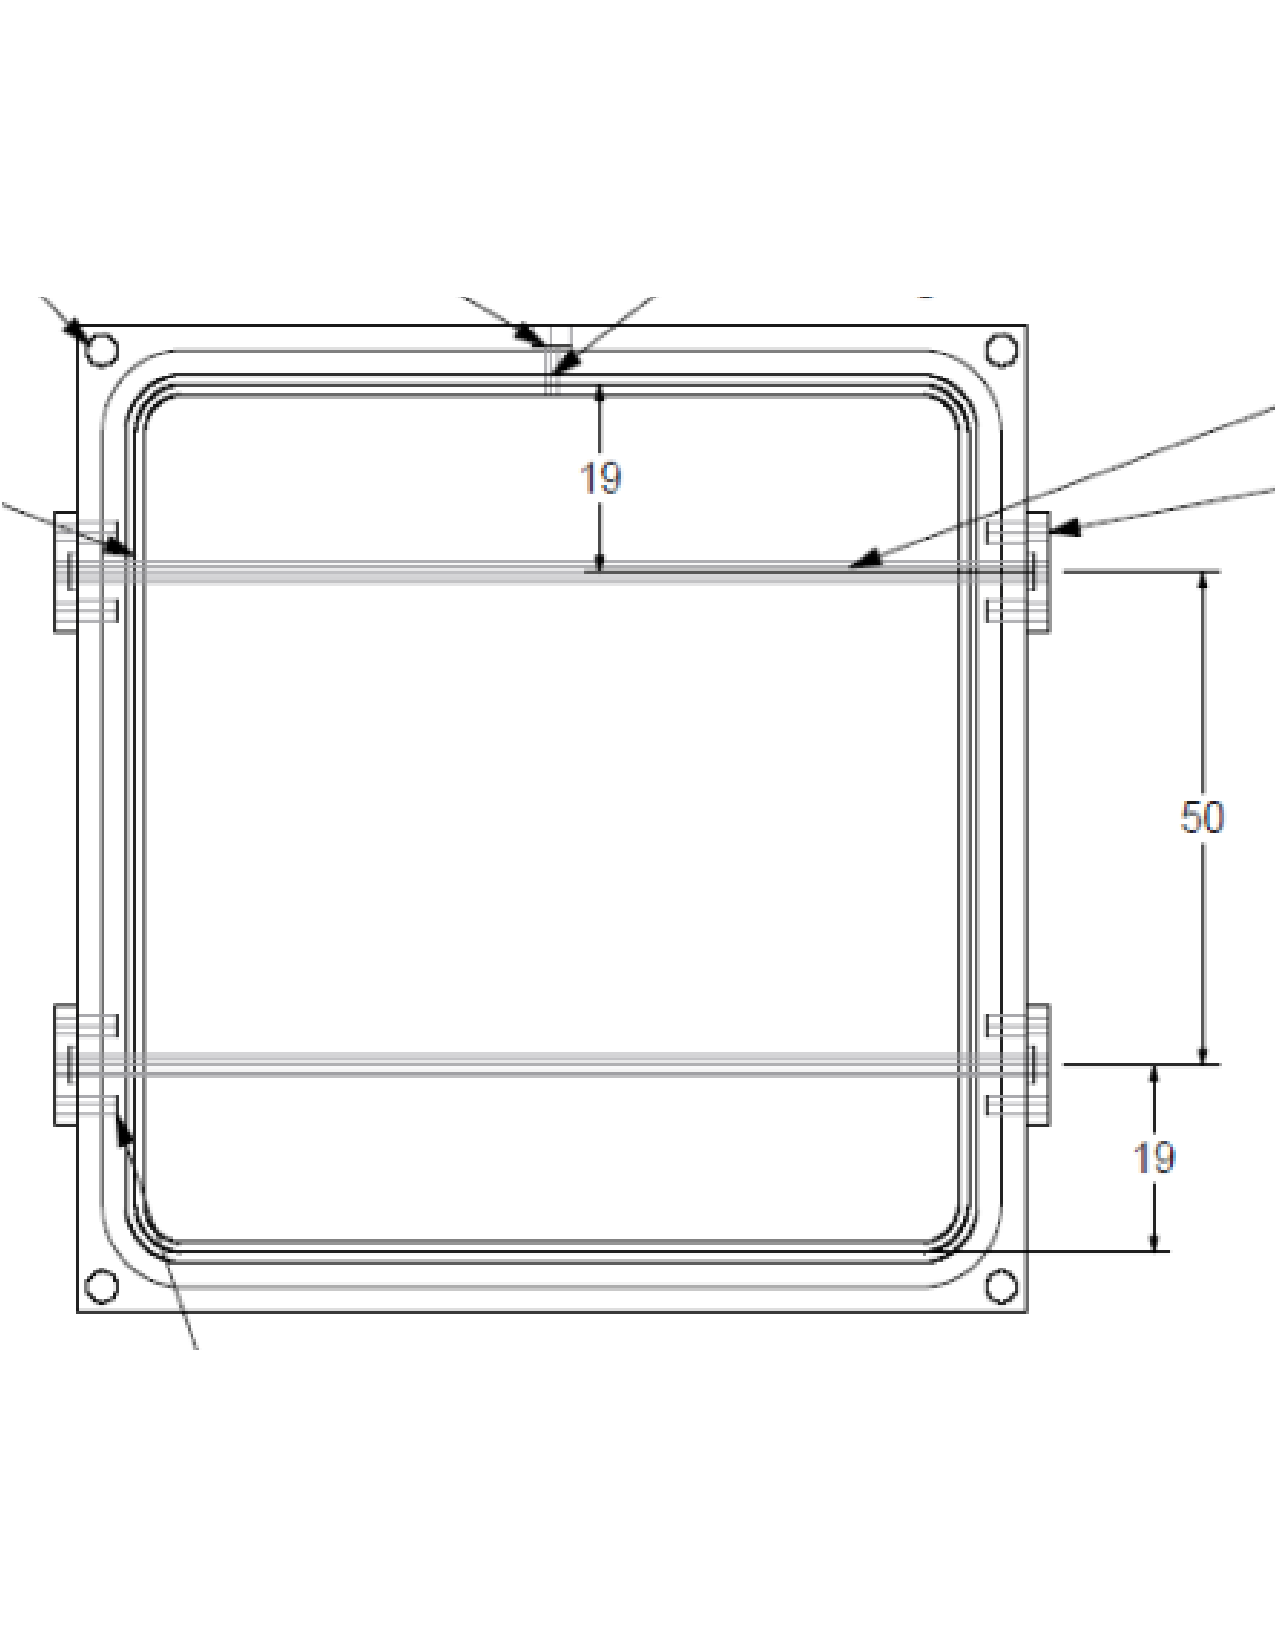
\includegraphics[width=0.8\textwidth]{mechanicaldesign.pdf}
\caption{
Mechanical design of a liquid scintillator tile.  Units are mm.
}
\label{fig:tiledesign}
\end{center}
\end{figure}



\section{Test beam results}

The light yield and uniformity of the tiles was measured in the H2 test beam facility at CERN using 120 GeV muons.

\section{Light yield dependence on tile parameters and comparison with simulation}
We use the GEANT4~\cite{Agostinelli2003250} package to simulate the optics of our tile.  

\section{Radiation hardness tests}

Several different tests were made using irradiations with a $\rm{^{60}Co}$ source lcoated at the University of Maryland.  Performance of the tile under irradiation in a proton-proton collision environment will be the subject of a future paper.

\section{Conclusions}

\section{Acknowledgements}
The authors would like to thank Randy Ruchti of Notre Dame for providing the capillaries and Yasar Onel's group at the University of Iowa for help with the test beam.  We would like to thank Eric Johnston from the Quattrone Nanofabrication Facility  at the University of Pennsylvania for measuring the indices of refraction of our support tubes.
This work was supported in part by U.S. Department of Energy Grant YYYYY.

\section*{References}

\bibliography{aliquidtile}

\end{document}
